%%% Local Variables:
%%% mode: latex
%%% TeX-master: "../main"
%%% End:
\newcommand{\flux}[1]{L_#1(\pmb{x}, \vec{\omega_o})}


\section{Introduction}

\begin{frame}
  \frametitle{Rendering Translucent Materials}
  \only<1>{\begin{figure}[!ht]
    \centering
    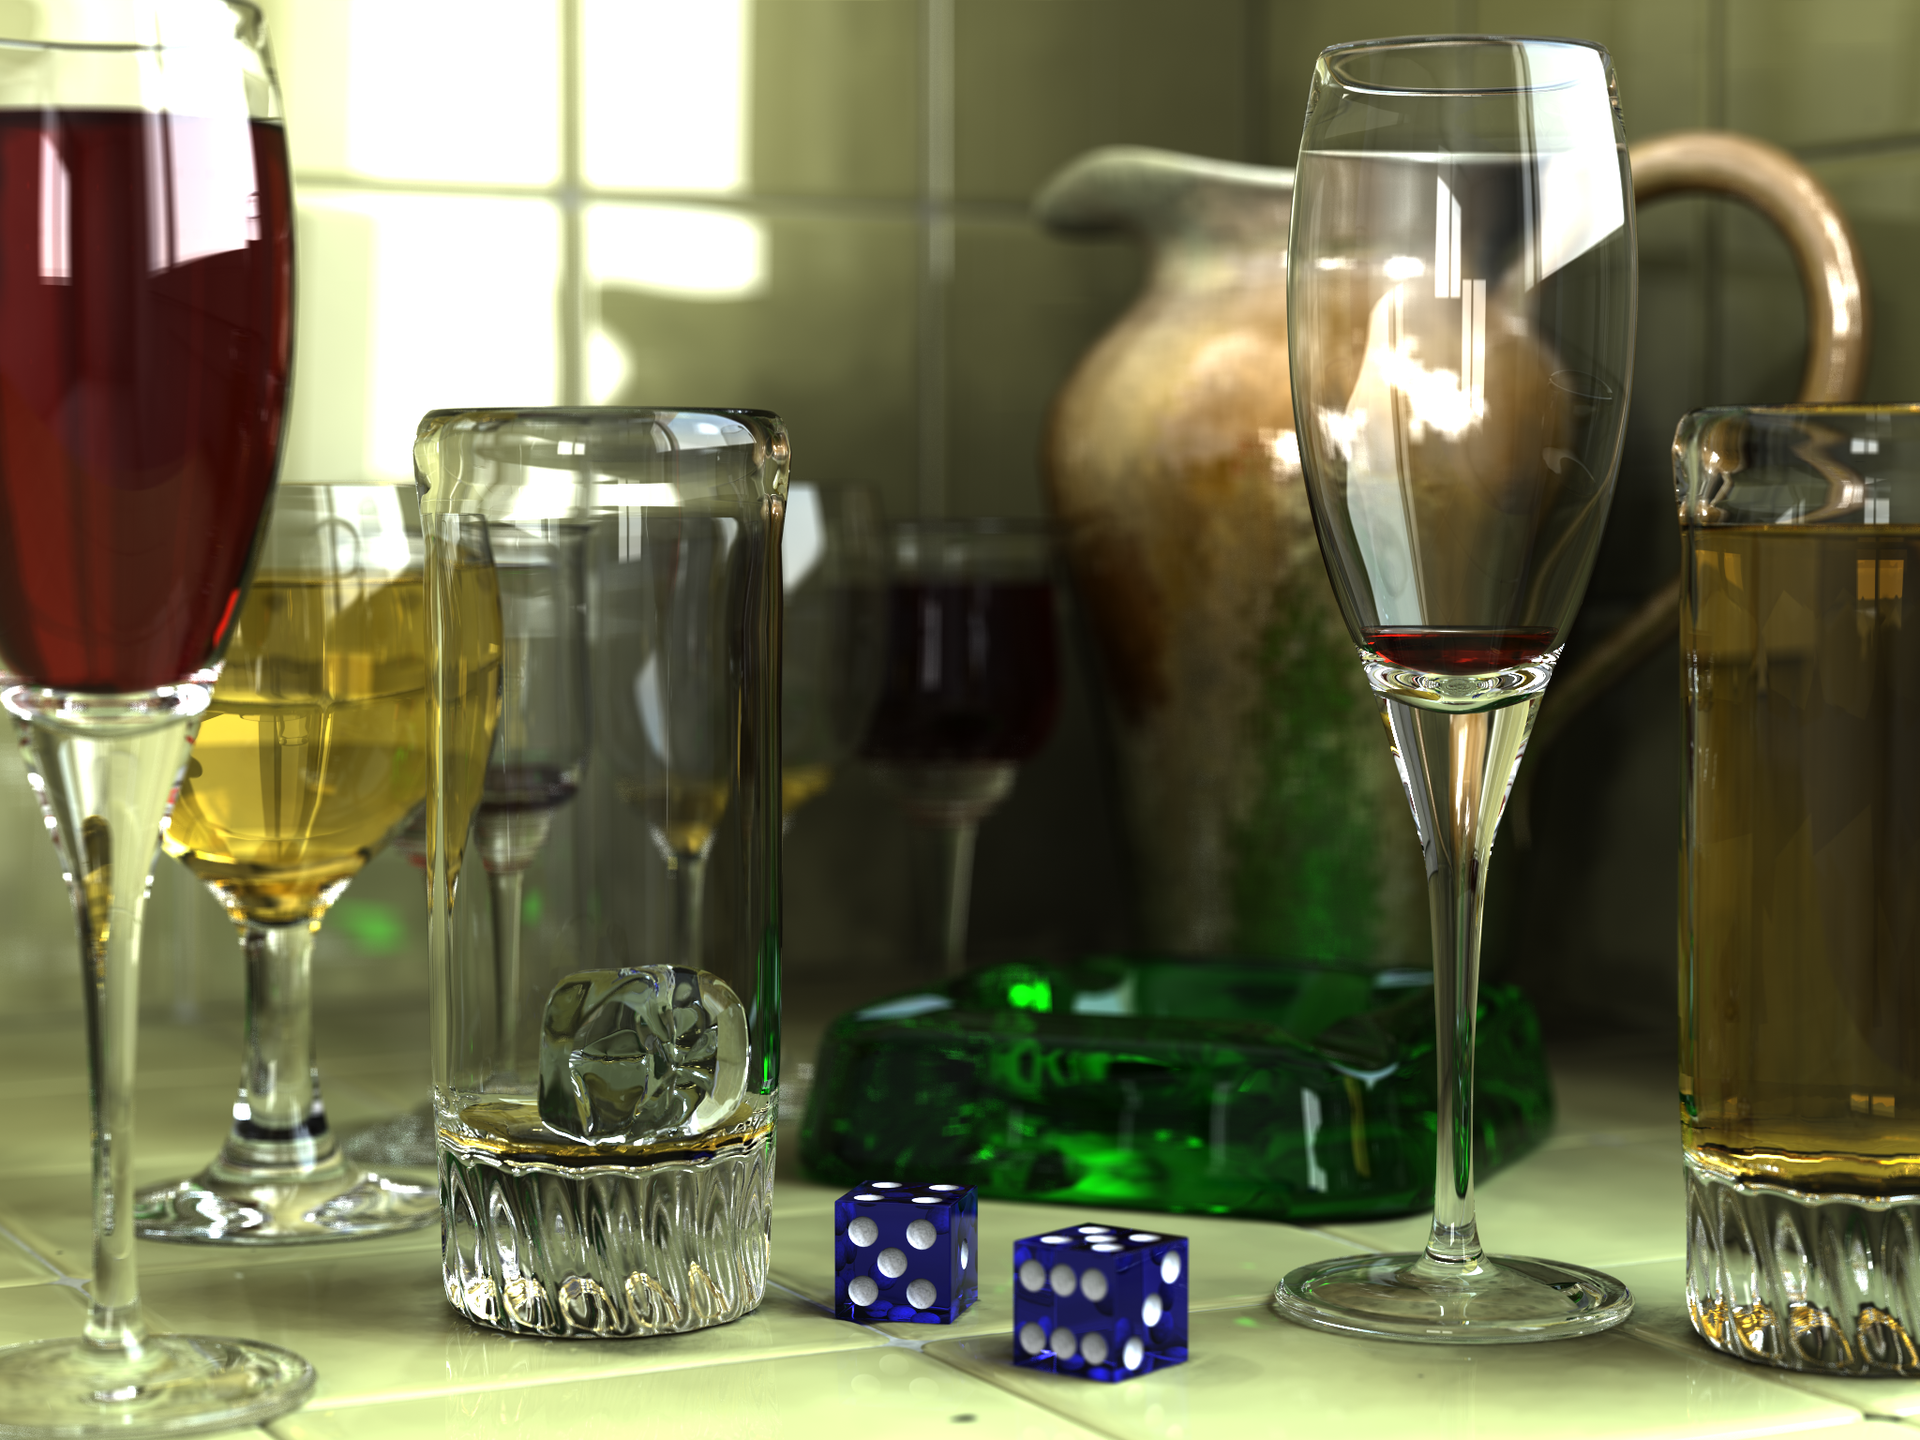
\includegraphics[scale=0.15]{renering.png}
  \end{figure}
}
\only<2>{
  \begin{figure}[!ht]
    \centering
    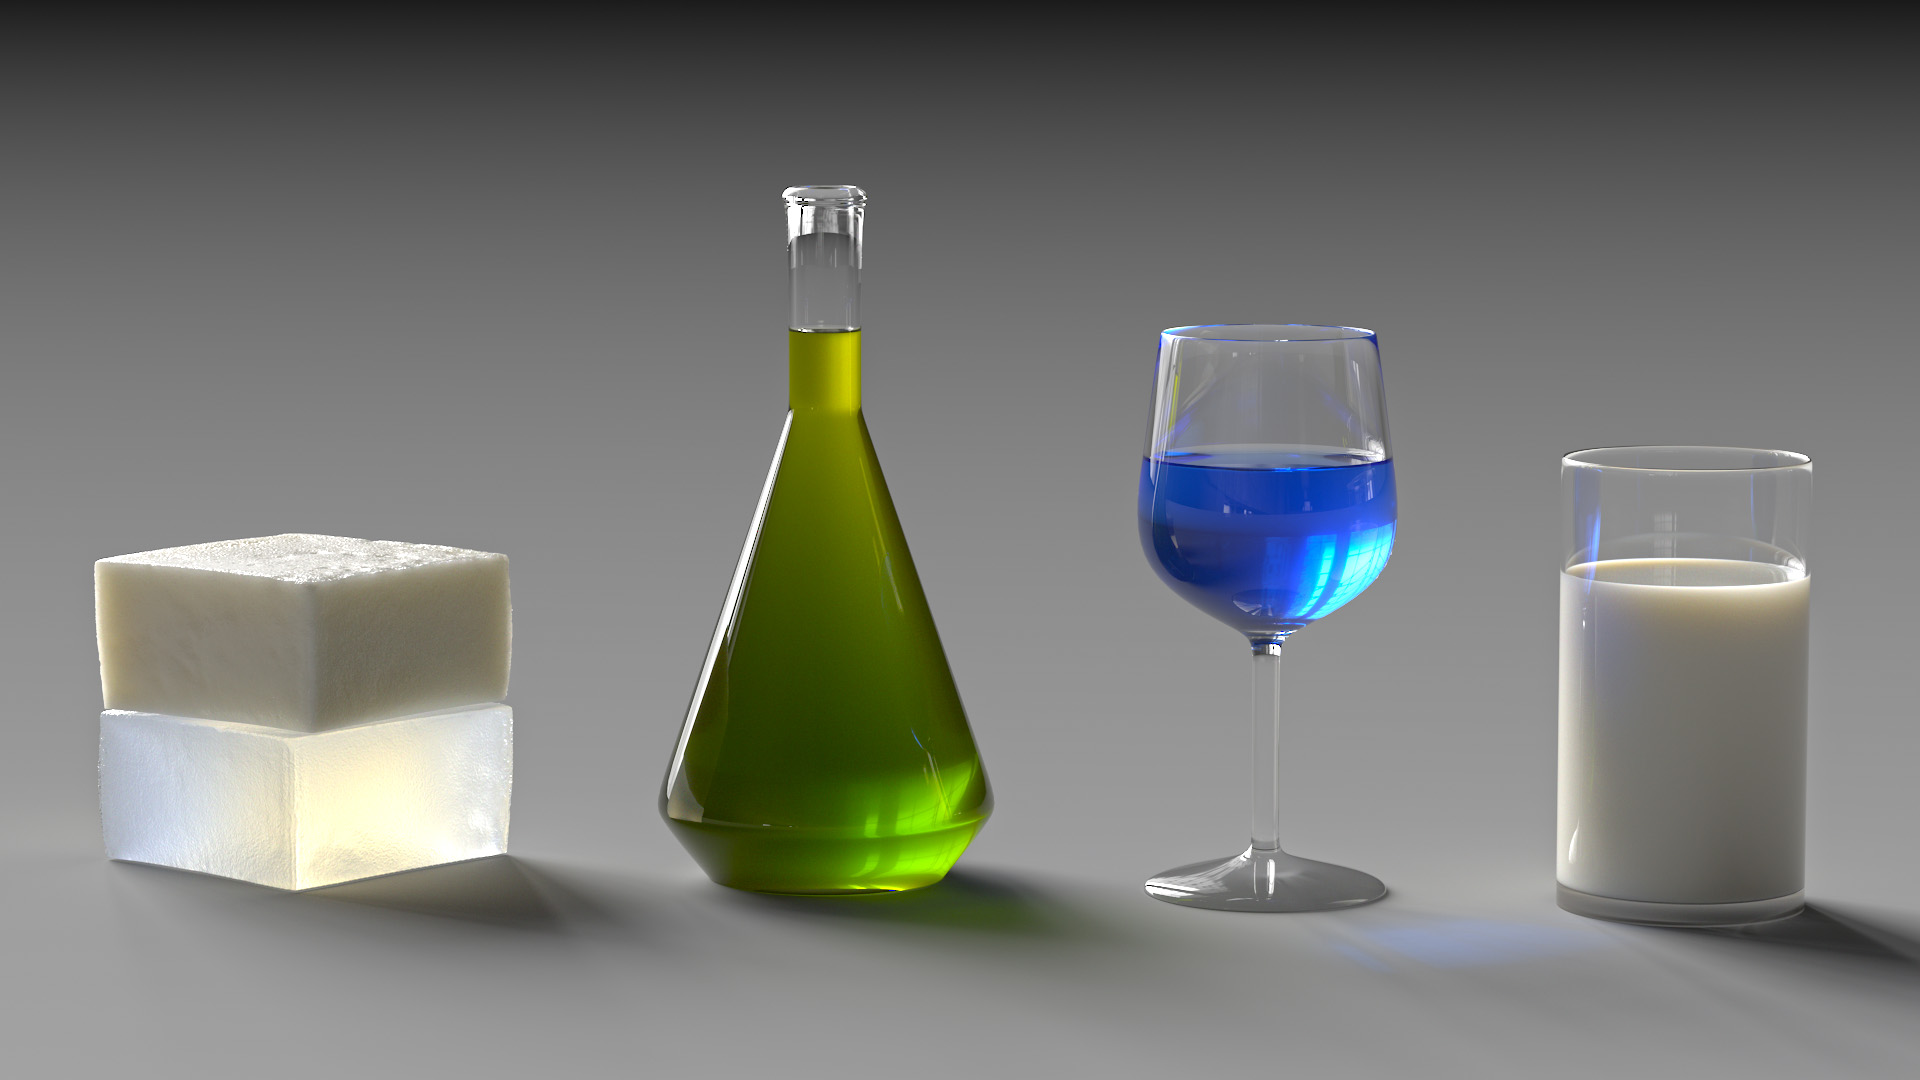
\includegraphics[scale=0.16]{trans.jpg}
  \end{figure}
}

\end{frame}


\section{BSSRDF}
\begin{frame}
  \frametitle{Light Transmission Models}
\only<1>{\begin{figure}[!ht]
    \centering
    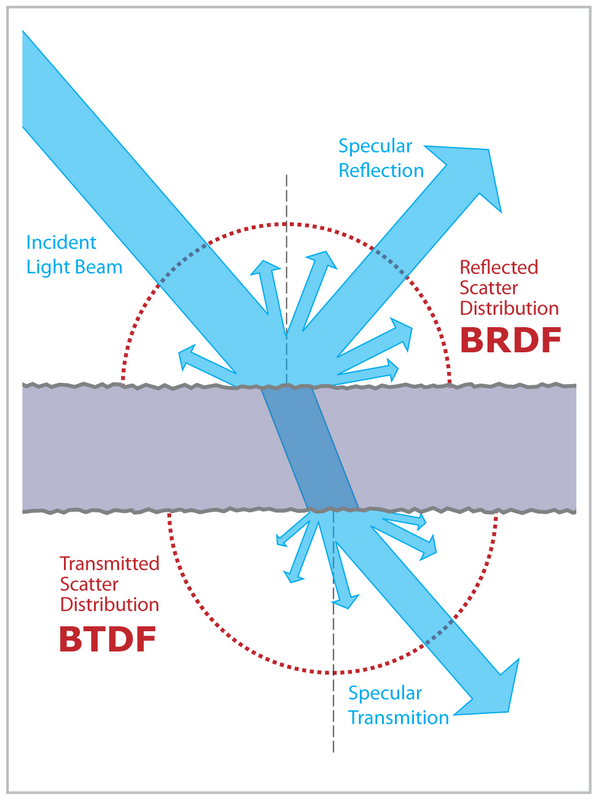
\includegraphics[scale=0.25]{bsdf.png}
  \end{figure}
}
\only<2>{
\begin{figure}[!ht]
    \centering
    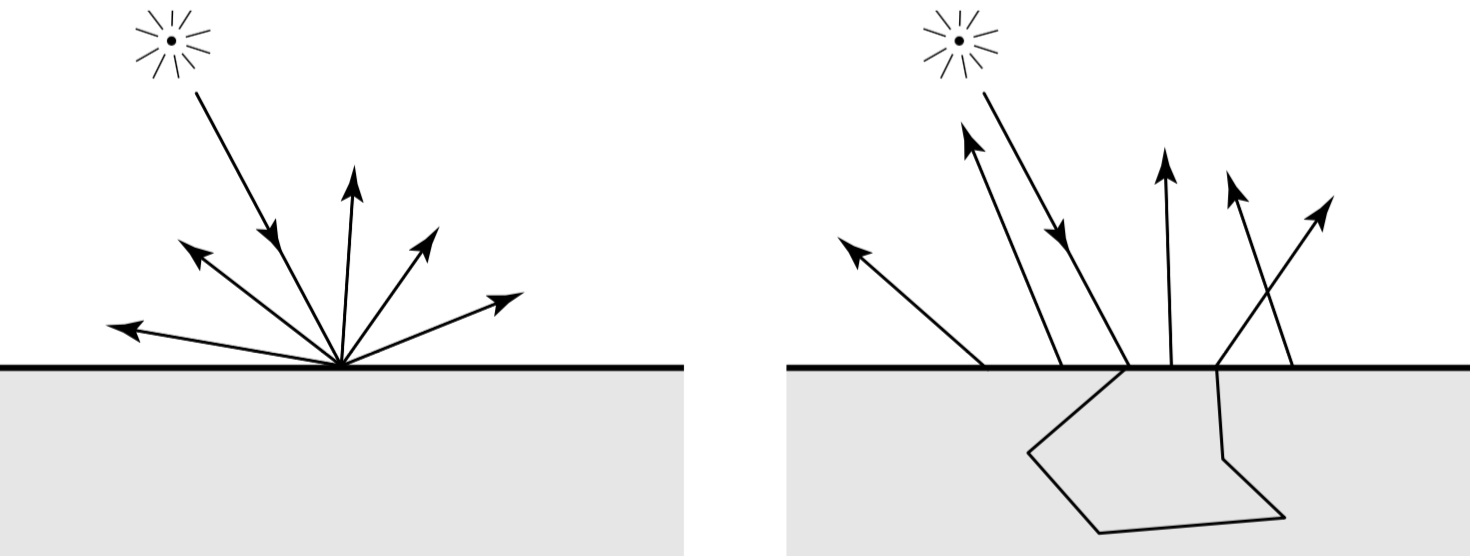
\includegraphics[scale=0.4]{bsdfbssrdf.png}
    \caption{Two models to describe the light transmission in
      translucent materials.}
  \end{figure}

}
\end{frame}



\begin{frame}
  \frametitle{Dipole Method}
  \begin{figure}[!ht]
    \centering
    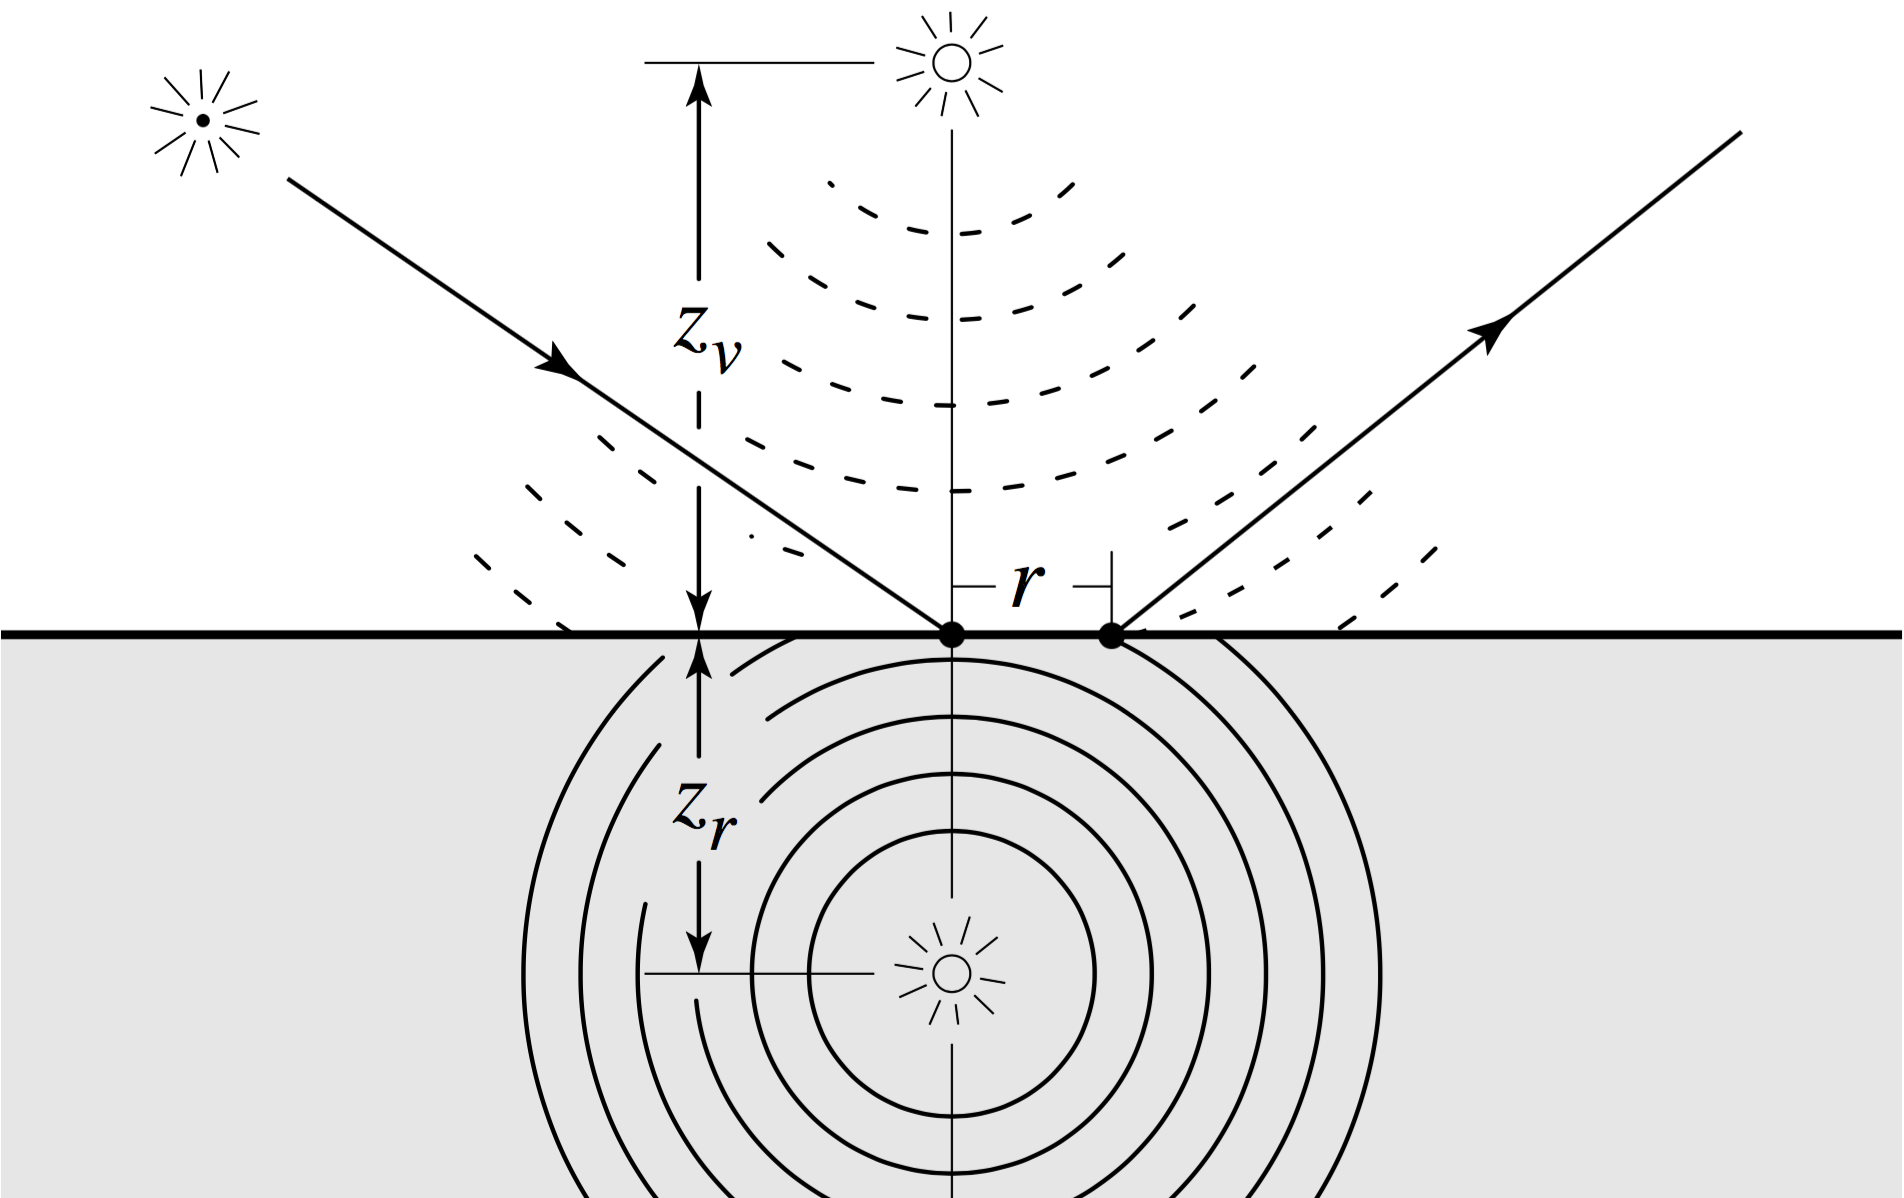
\includegraphics[scale=0.15]{di.png}
    \hspace{4mm}
    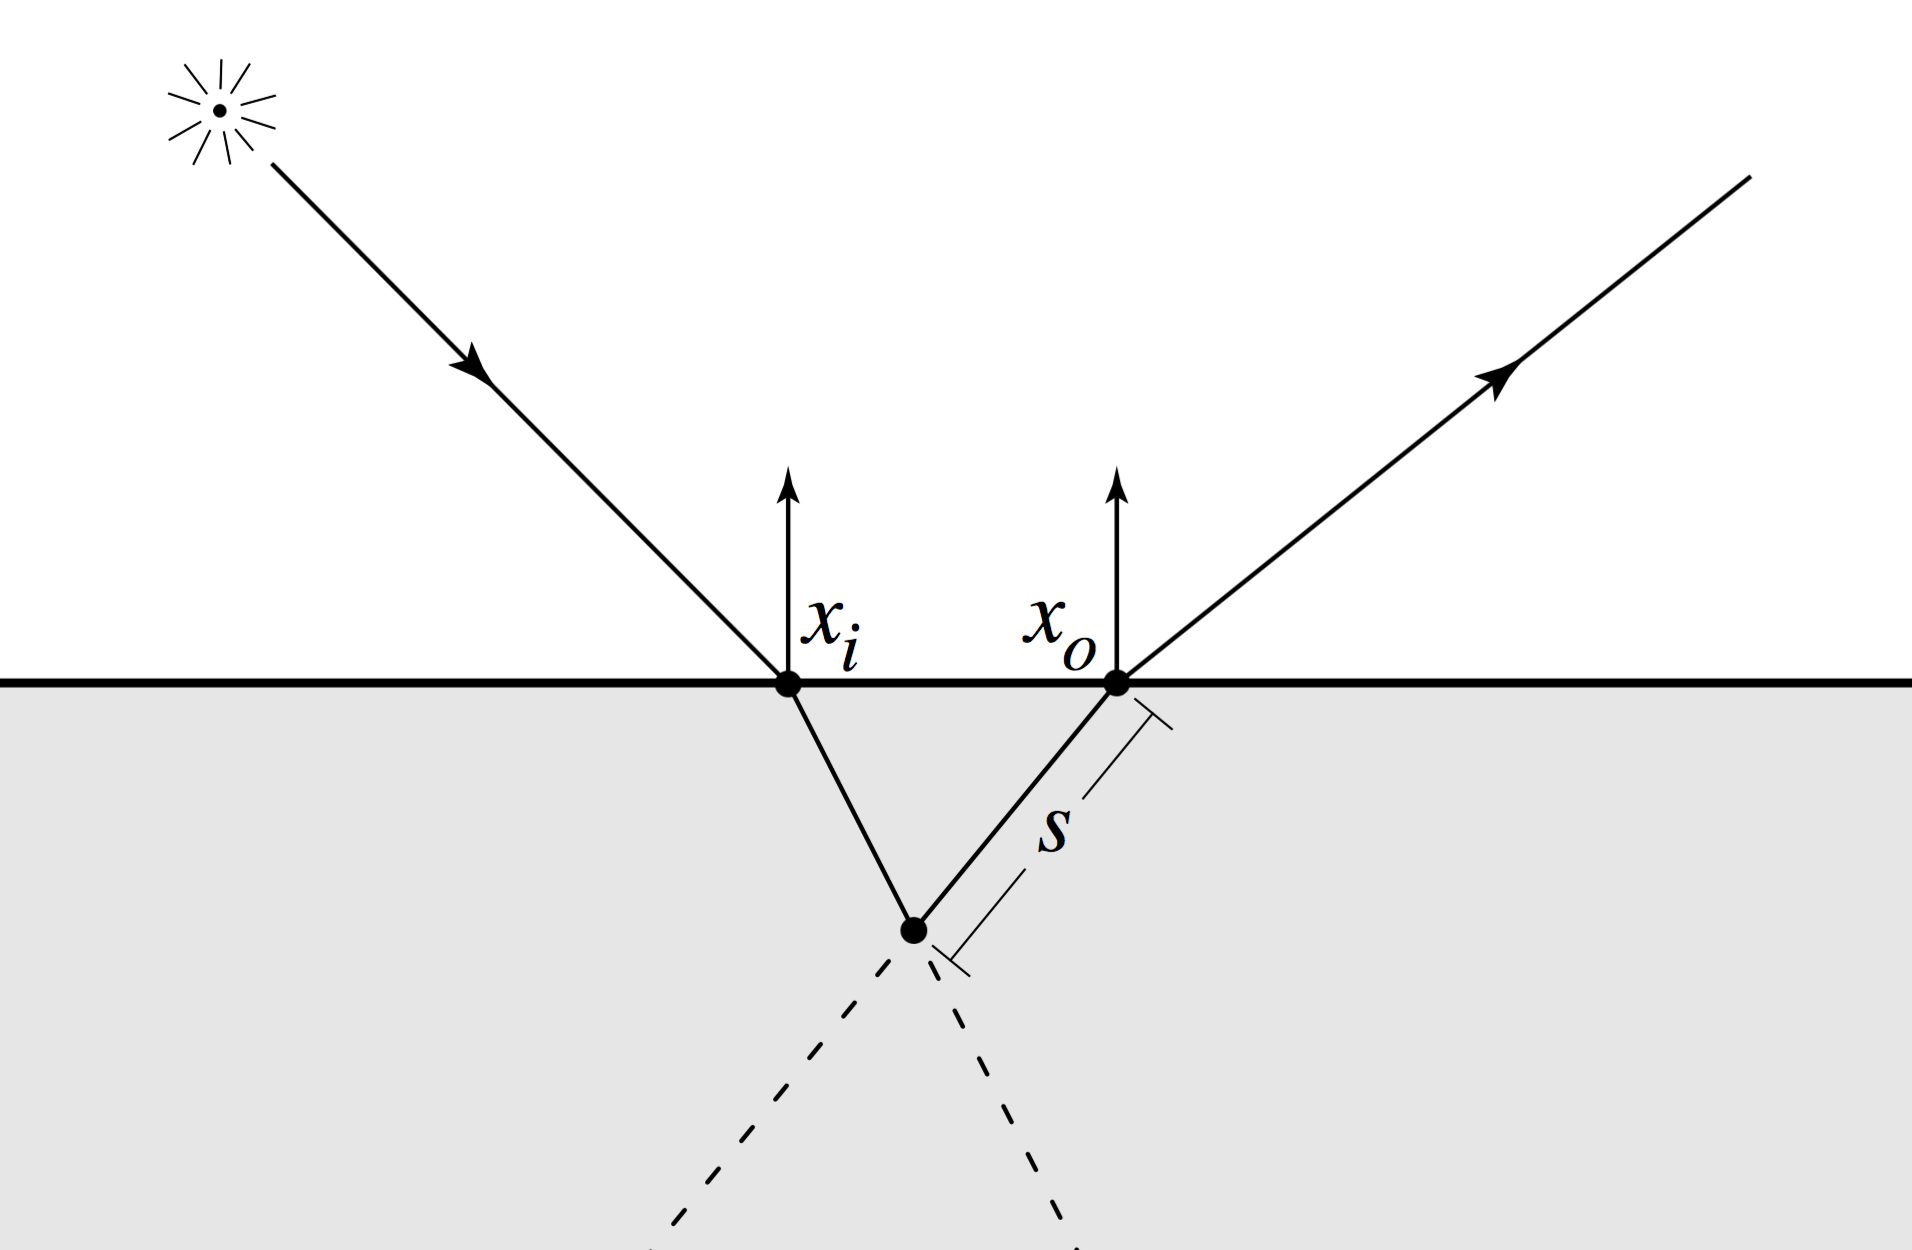
\includegraphics[scale=0.15]{single.png}
  \end{figure}
\end{frame}

\begin{frame}
  \frametitle{BSSRDF Rendering}
Rendering translucent material takes a little bit more effort:

  \begin{align*}
\flux{o} &= \flux{e} + \flux{r} = \flux{e}\\
         & + \int_A\int_{2\pi}S(x_i, \vec{\omega_i}; x_o,
           \vec{\omega_o})L_i(\pmb{x}, \vec{\omega})(\vec{\omega}\cdot\vec{n})d\omega_idA
  \end{align*}

and

$$
S(x_i, \vec{\omega_i}; x_o, \vec{\omega_o})  = S_d(x_i,
\vec{\omega_i}; x_o, \vec{\omega_o}) +S^{(1)}(x_i, \vec{\omega_i};
x_o, \vec{\omega_o})
$$

where $S$ is BSSRDF. $S_d$ and $S^{(1)}$ are the{\bf  diffusion approximation} and
{\bf single scattering term}.

\end{frame}


\section{Directional Dipole}

\begin{frame}
  \frametitle{Dipole Methods}
  \begin{figure}[!ht]
    \centering
    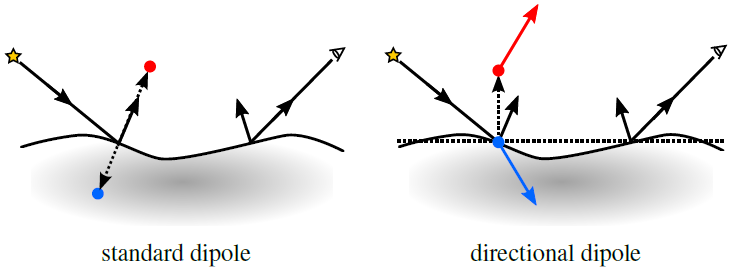
\includegraphics[scale=0.55]{dipoles.png}
  \end{figure}
\end{frame}

\begin{frame}
  \frametitle{Basic Implementation}
  \begin{figure}[!ht]
    \centering
    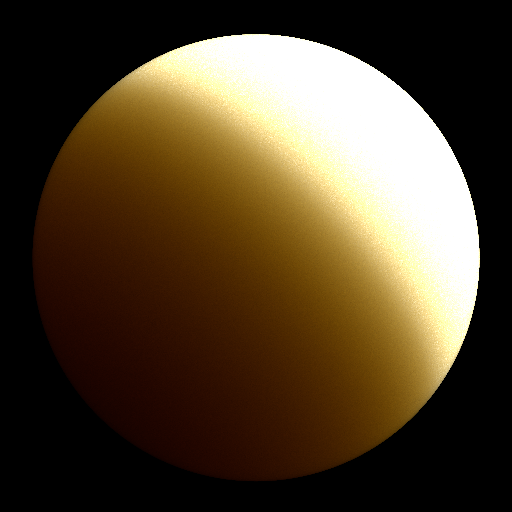
\includegraphics[scale=0.4]{render.png}
  \end{figure}

\end{frame}
